\documentclass{beamer}
\usepackage[utf8]{inputenc}
\usepackage{graphicx}
\usetheme{AnnArbor}
\useinnertheme[shadow=true]{rounded}

\title[Física em um Passeio de Bicicleta]{Física em um passeio de Bicicleta
}
\author[Victor Nunes]{Victor Santos Nunes\inst{1}}
\institute[DFI-UFS]{
	\inst{1}
	Departamento de Física\\
	Universidade Federal de Sergipe	
}
\date[2019]{2019}
	
\begin{document}
	\frame{\titlepage}
	
	\begin{frame}
		\frametitle{Sumário}
		\tableofcontents
	\end{frame}
	
	\begin{frame}
		\frametitle{Avisos}
		\begin{itemize}
			\item Sem vínculo com a UFS
			\item Eu sou um teórico, perdoem-me
			\item Me impeçam de enlouquecer vocês
		\end{itemize}
	\end{frame}
	
	\begin{frame}
		\frametitle{Antes de tudo, quem sou eu ?}
		\begin{itemize}
			\item<1-> Técnico em Eletrônica (IFS),
			\item Bacharelando em Astrofísica (UFS),
			\item Bacharelando em Engenharia Mecatrônica (Trancado no 4º Período) (UNIT),
			\item Pesquisador de Matemática (DMA-UFS),
			\item Ex-pesquisador de novos materiais para Manufatura Aditiva (UNIT),
			\item Ex-integrante do sistema de Elétrica/Eletrônica/Computação da equipe Serbaja (DMEC-UFS),
			\item Estudante associado à SAE (Sociedade de Engenheiros da Mobilidade),
			\item<2-> Estagiário em Análise de Dados e Inteligência Artificial (Inventione).
		\end{itemize}
	\end{frame}

	\begin{frame}
		\frametitle{Agora, quem eu era !}
		Mostrar Médias
	\end{frame}

	\begin{frame}
	\section{O que é Física ?}
		\frametitle{O que é Física ?}
		\begin{figure}[h]
			\centering
			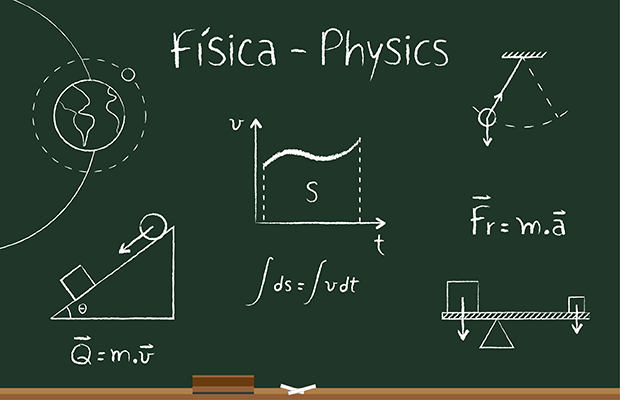
\includegraphics[scale=0.5]{physics.png}
			\label{What a hell is physics ?}
		\end{figure}
	\end{frame}

	\begin{frame}
		\frametitle{What the hell is Theoretical Physics?}
		\begin{figure}[h]
			\centering
			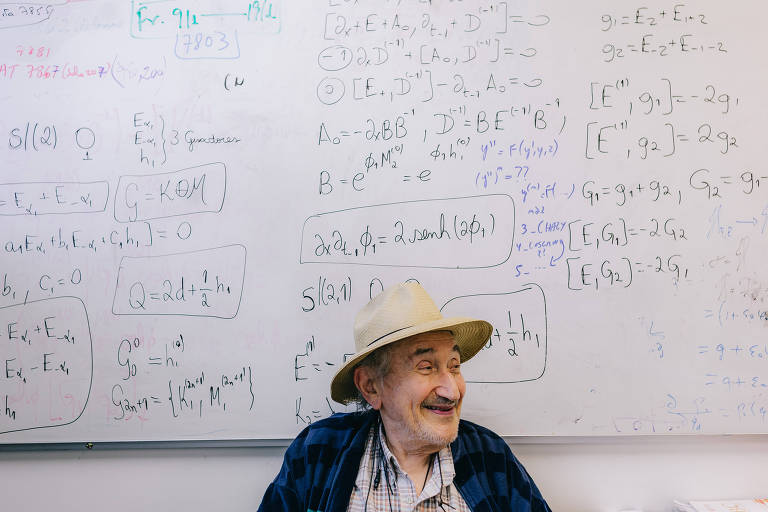
\includegraphics[scale=1.6]{teorica.jpg}
		\end{figure}
	\end{frame}
	
	\begin{frame}
		\frametitle{Experimental Physics ?!?!}
		\begin{figure}[h]
			\centering
			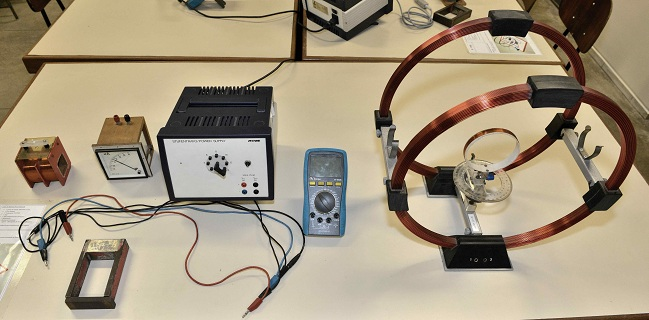
\includegraphics[scale=2]{experimental.jpg}
		\end{figure}
	\end{frame}
	\begin{frame}
		\section{Como a bicicleta se mantém em pé ?}
		\frametitle{Como a bicicleta se mantém em pé ?}
		\begin{figure}[h]
			\centering
			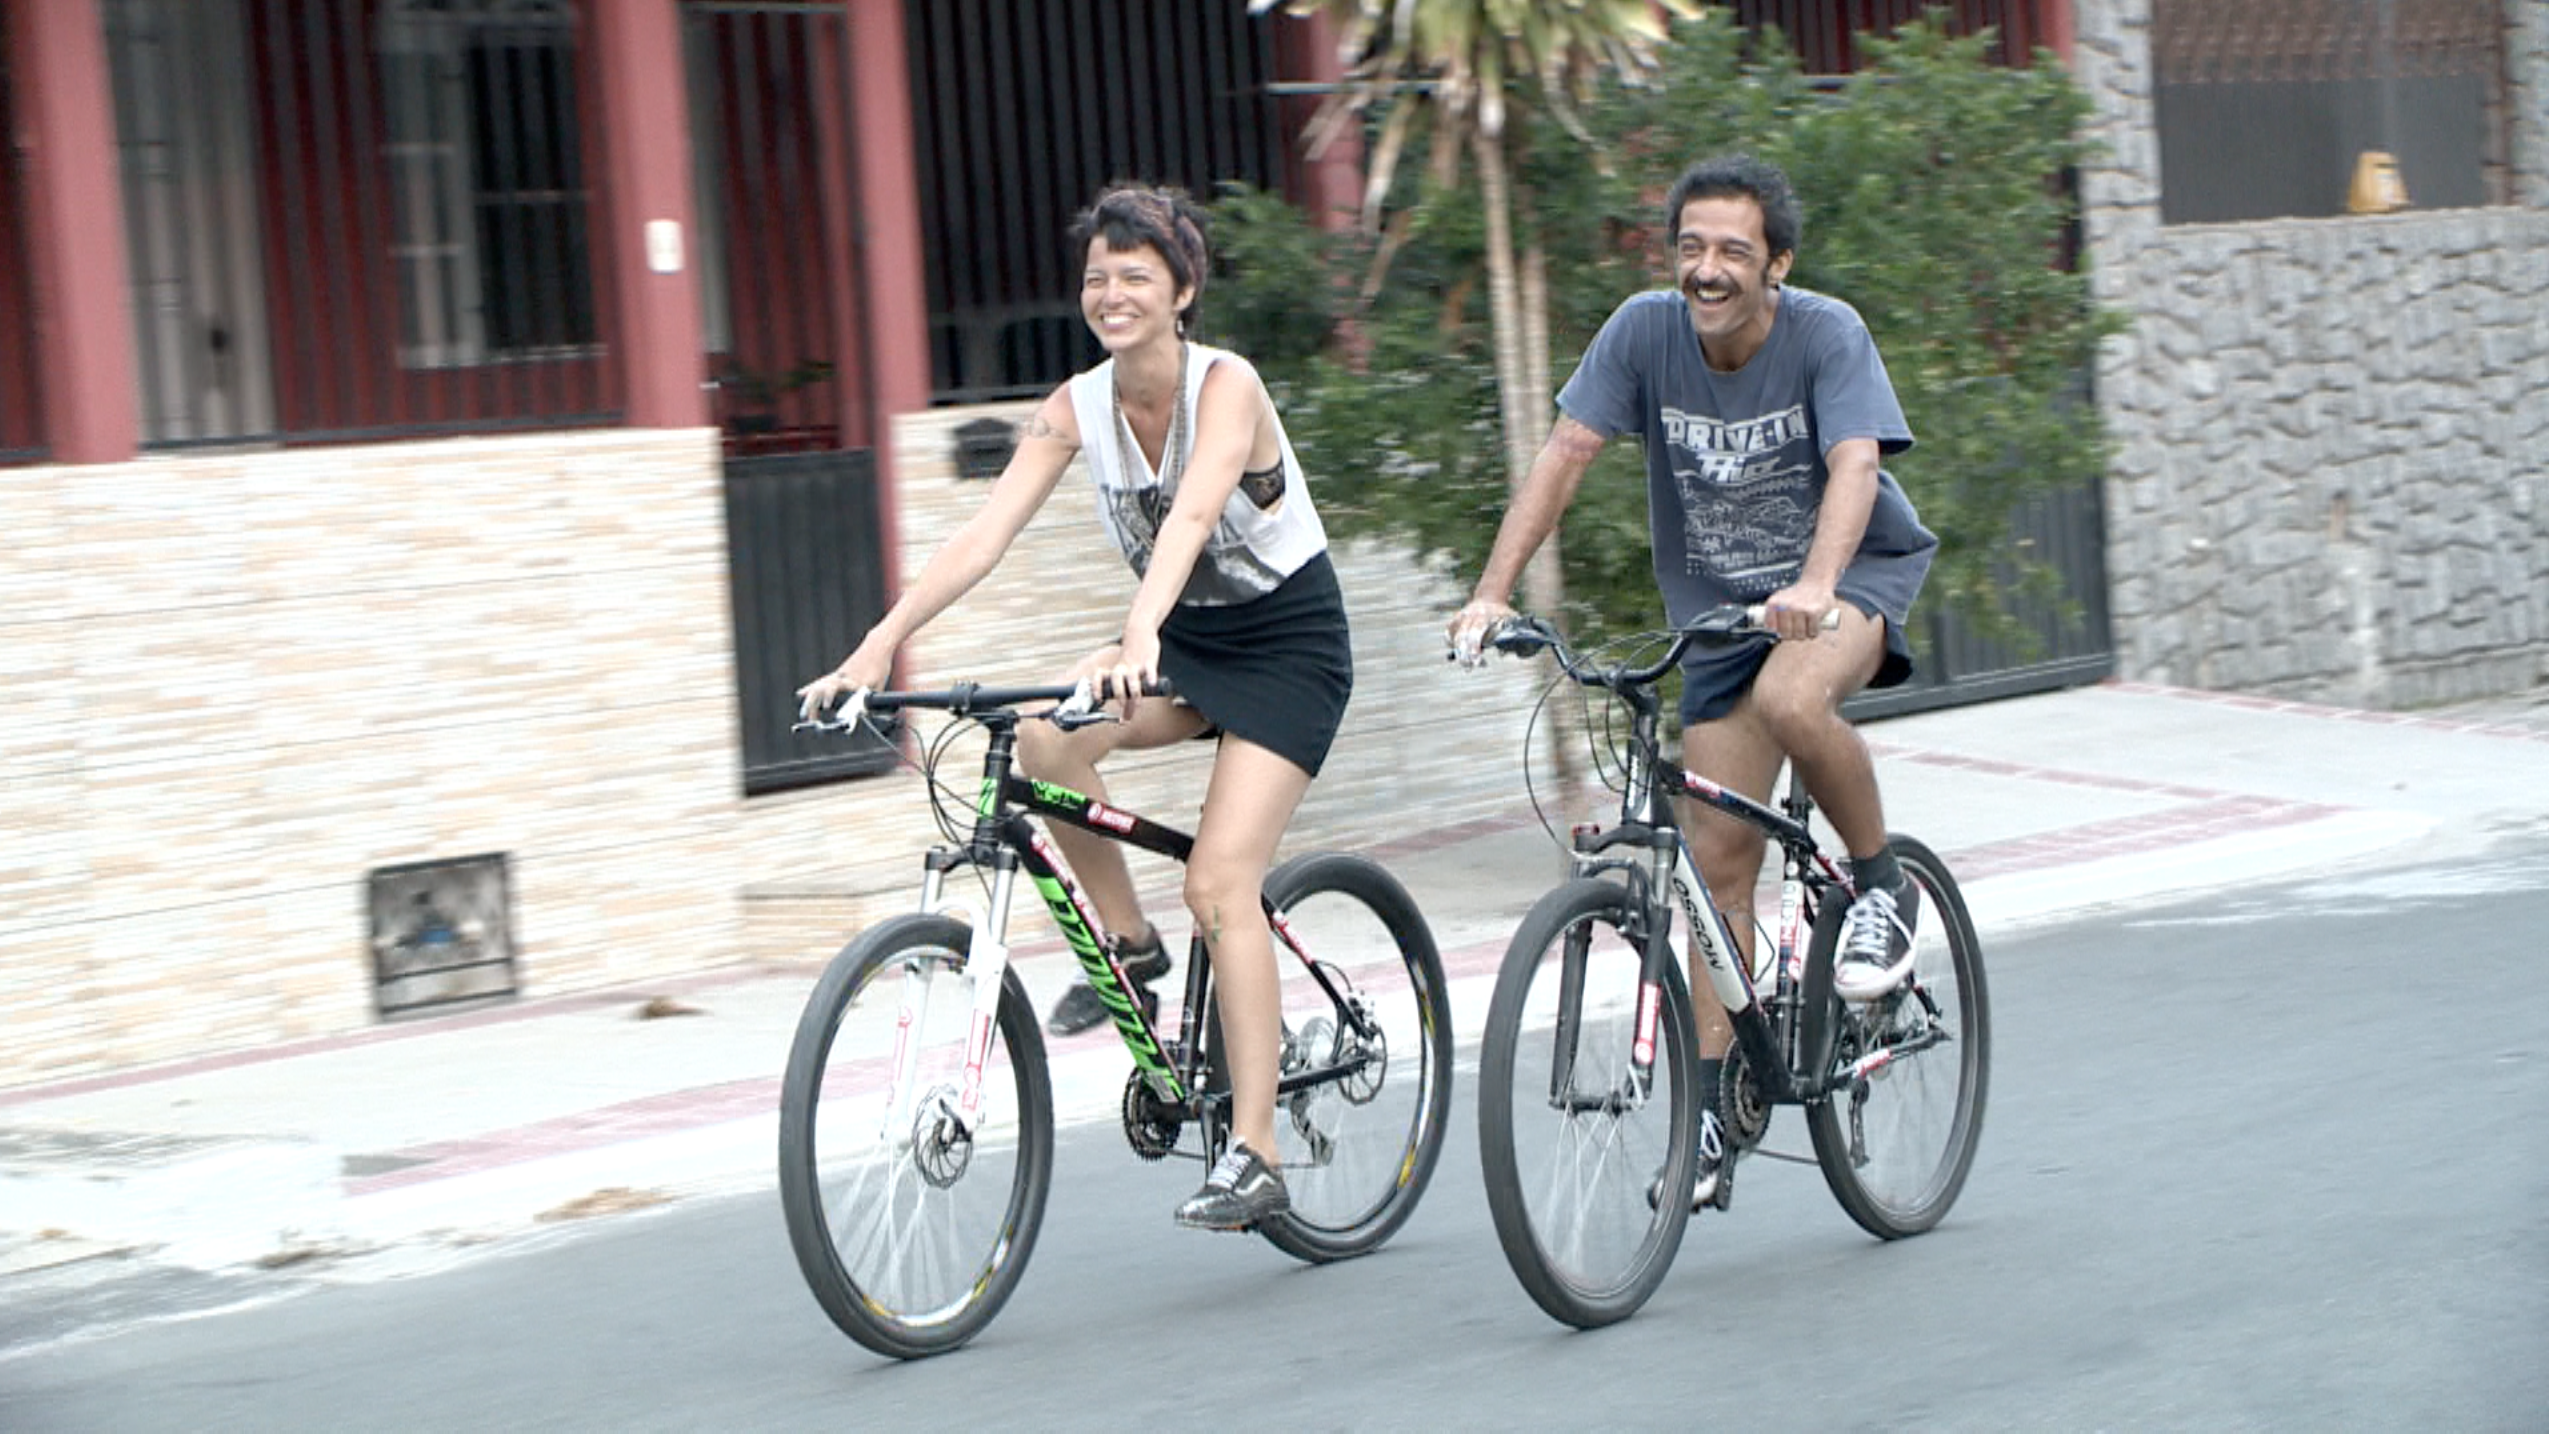
\includegraphics[scale=0.13]{bike.png}
		\end{figure}
	\end{frame}

	\begin{frame}
		\section{Trocando o pneu}
		\frametitle{Trocando o pneu}
		\begin{figure}[h]
			\centering
			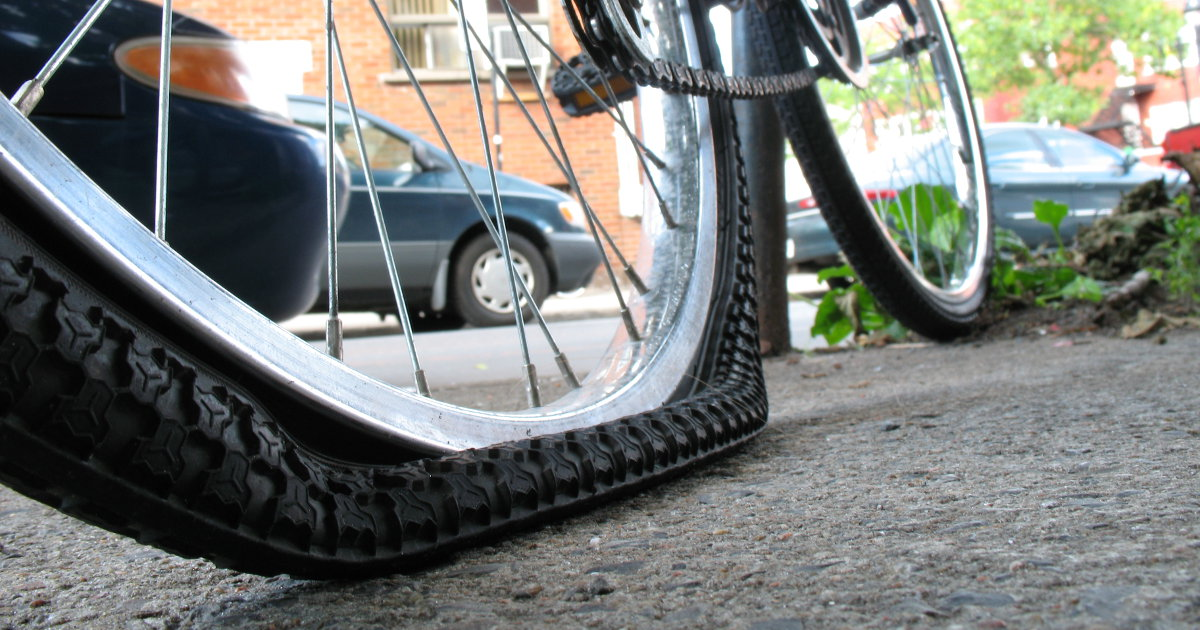
\includegraphics[scale=0.7]{pneufurado.jpg}
		\end{figure}
	\end{frame}
	
	\begin{frame}
		\section{Calibrando o pneu}
		\frametitle{Calibrando o pneu}
		\begin{figure}[h]
			\centering
			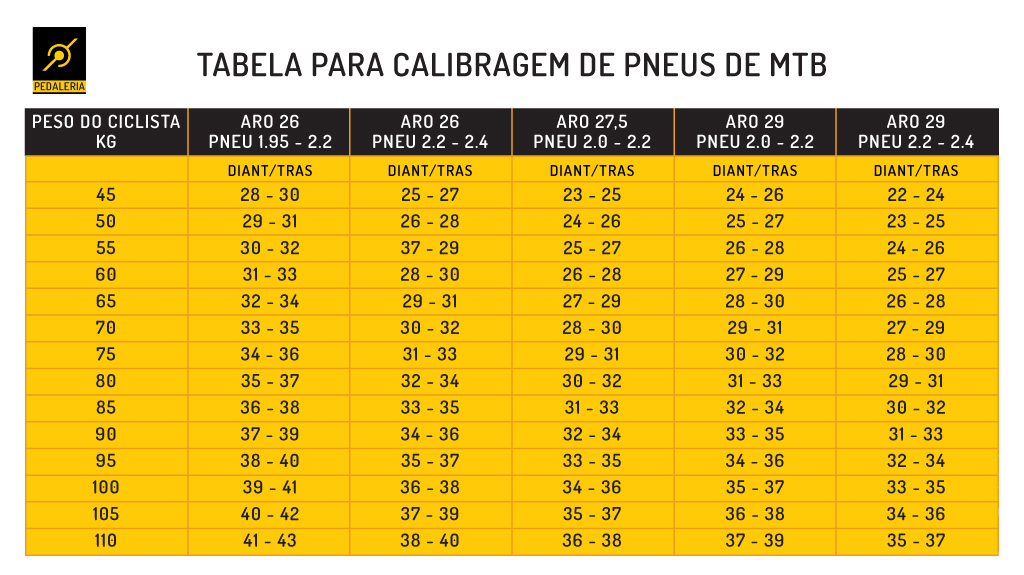
\includegraphics[scale=0.3]{mtb.jpg}
		\end{figure}
	\end{frame}
	
	\begin{frame}
		\frametitle{Calibrando o pneu}
		\begin{figure}[h]
			\centering
			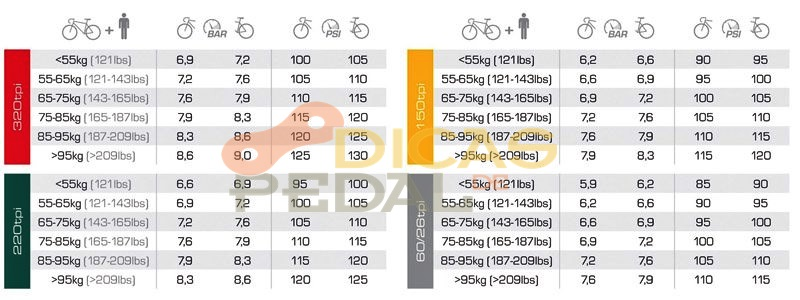
\includegraphics[scale=0.5]{speed.jpg}
		\end{figure}
	\end{frame}
	
		\begin{frame}
	\section{Calibrando o pneu}
	\frametitle{Calibrando o pneu}
	\begin{figure}[h]
		\centering
		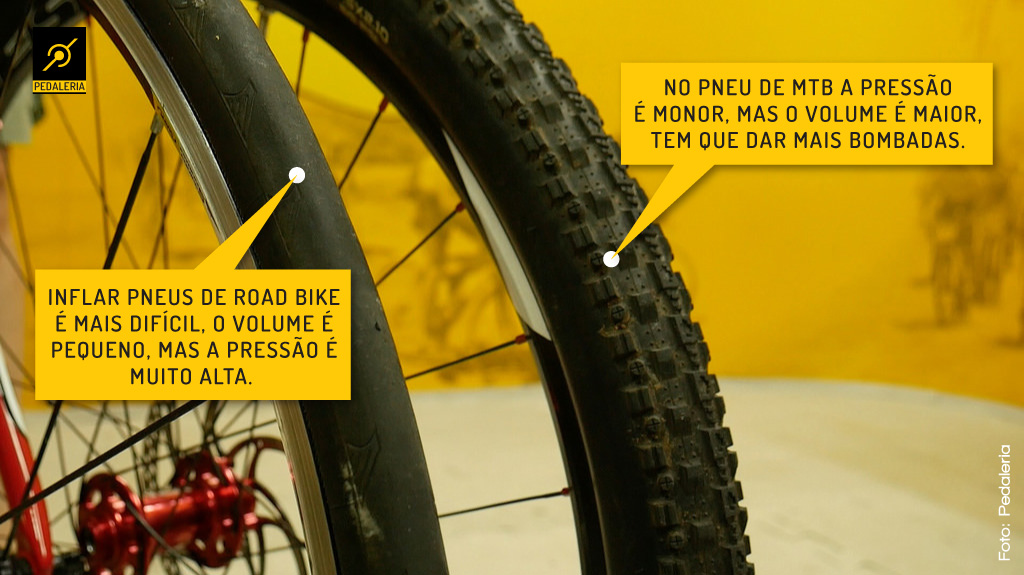
\includegraphics[scale=0.3]{mtbxspeed.jpg}
	\end{figure}
\end{frame}
	
	\begin{frame}
		\section{Como a bicicleta faz curva ?}
		\frametitle{Como a bicicleta faz curva ?}
		Precessão do Giroscópio
	\end{frame}

	\begin{frame}
		\section{Colisões com bicicletas}
		\frametitle{Colisões com bicicletas}
		Momento, \\
		Conservação de Momento, \\
		Colisões
	\end{frame}

	\begin{frame}
		\section{Como o freio freia ? ashashaha}
		\frametitle{Como o freio freia ?}
		Noções de alavanca, \\
		Atrito, \\
		Conversão de Energia
	\end{frame}

	\begin{frame}
		\section{Descendo uma ladeira (ou rampa)}
		\frametitle{Descendo uma ladeira (ou rampa)}
		Noções de Conservação de Energia, \\
		Resolução de problemas com análise de forças, \\
		Forças Dissipativas
	\end{frame}

	\begin{frame}
		\section{Como funcionam as marchas da bicicleta}
		\frametitle{Como funcionam as marchas da bicicleta}
		Engrenagens, \\
		Polias, \\
		MCU
	\end{frame}

	\begin{frame}
		\section{Física das manobras}
		\frametitle{Física das manobras}
		Centro de massa e gravidade
	\end{frame}

\end{document}